In short, we find that the feature-based clustering discerned two
meaningfully different groups of participants. We find an adaptive group
(cluster 1) that reports higher well-being and more positive outgroup
attitudes (\textit{median}) that are also stable over time
(\textit{MAD}, \textit{MAC}) and tend to increase over the 30 day test
period (\textit{linear trend}). This group also reported consistently
more meaningful, need-fulfilling, and cooperative outgroup interactions
(\textit{median}). This group with overwhelmingly positive experiences
stands in contrast with a more detrimental group (cluster 2). This
cluster, on average, reported much less positive, less meaningful, and
less fulfilling interactions and interaction patterns (\textit{median}).
This group also reported less positive outgroup attitudes, lower
well-being, and more discrimination experiences (\textit{median}). At
the same time, for members of this detrimental cluster (cluster 2)
conditions seemed to deteriorate over time (\textit{linear trend}), and
there was generally less consistency in the experiences they were able
to have (\textit{MAC}, \textit{MAD}, \textit{edf}).

To identify these patterns, we first inspect the clusters based on the
average values of meaningful features (see
\fgrref[A]{fig:clusterFeatVar}; \citealp{Kennedy2021}). We see that for
some variables the features are generally stronger in separating the
clusters. We, for example, see that the item on
`\textit{how cooperative the interaction was}' distinguishes the two
clusters across almost all seven features (except for the
\textit{auto-correlation}, see \fgrref[A]{fig:clusterFeatVar}). Compare
this to the `\textit{outgroup attitudes}' item where the differences
between the clusters are much smaller for almost all features. We then
inspect the clusters with a focus on the features (see
\fgrref[B]{fig:clusterFeatVar}). While this is the same data as for the
variable focus, we can see more clearly that some features are better at
distinguishing the clusters across variables. For example, \textit{MAD}
and \textit{median} distinguish the two clusters across almost all
variables (except for the item of whether the interaction was
representative of the outgroup). These two features stand in stark
contrast to other features, such as the
\textit{lag-1 auto correlations}, which showed much smaller differences
between the two clusters (see \fgrref[B]{fig:clusterFeatVar}). This
offers some information on which features were most important in
understanding the two extracted groups. Taking these two perspectives
together, we can also focus on individual features or variables in
particular. We, for example, see a strong difference in the average
well-being, where participants in cluster 2 showed a much lower median
well-being over the time series. At the same time, in terms of
stability, both groups have virtually identical average \textit{MAC}
statistics for well-being (see \fgrref[A]{fig:clusterFeatVar}). There
are, thus, variables and features that distinguish the clusters better
than others and a combination of variables and features lets us explore
meaningful group differences in more detail. In our case, we see that
the central tendency, variability, and linear trend are best at
distinguishing a group with mainly positive experiences (cluster 1) from
a group with a more negative experience (cluster 2). We also see that
our clusters line up with the past literature on the importance of
focusing on simpler and more meaningful statistics
\citep{bringmann2018c, eronen2021a}.

\begin{figure}[!ht] %hbtp
  \caption{Cluster Group Comparisons based on Features and Variables}
  \label{fig:clusterFeatVar}
  \centering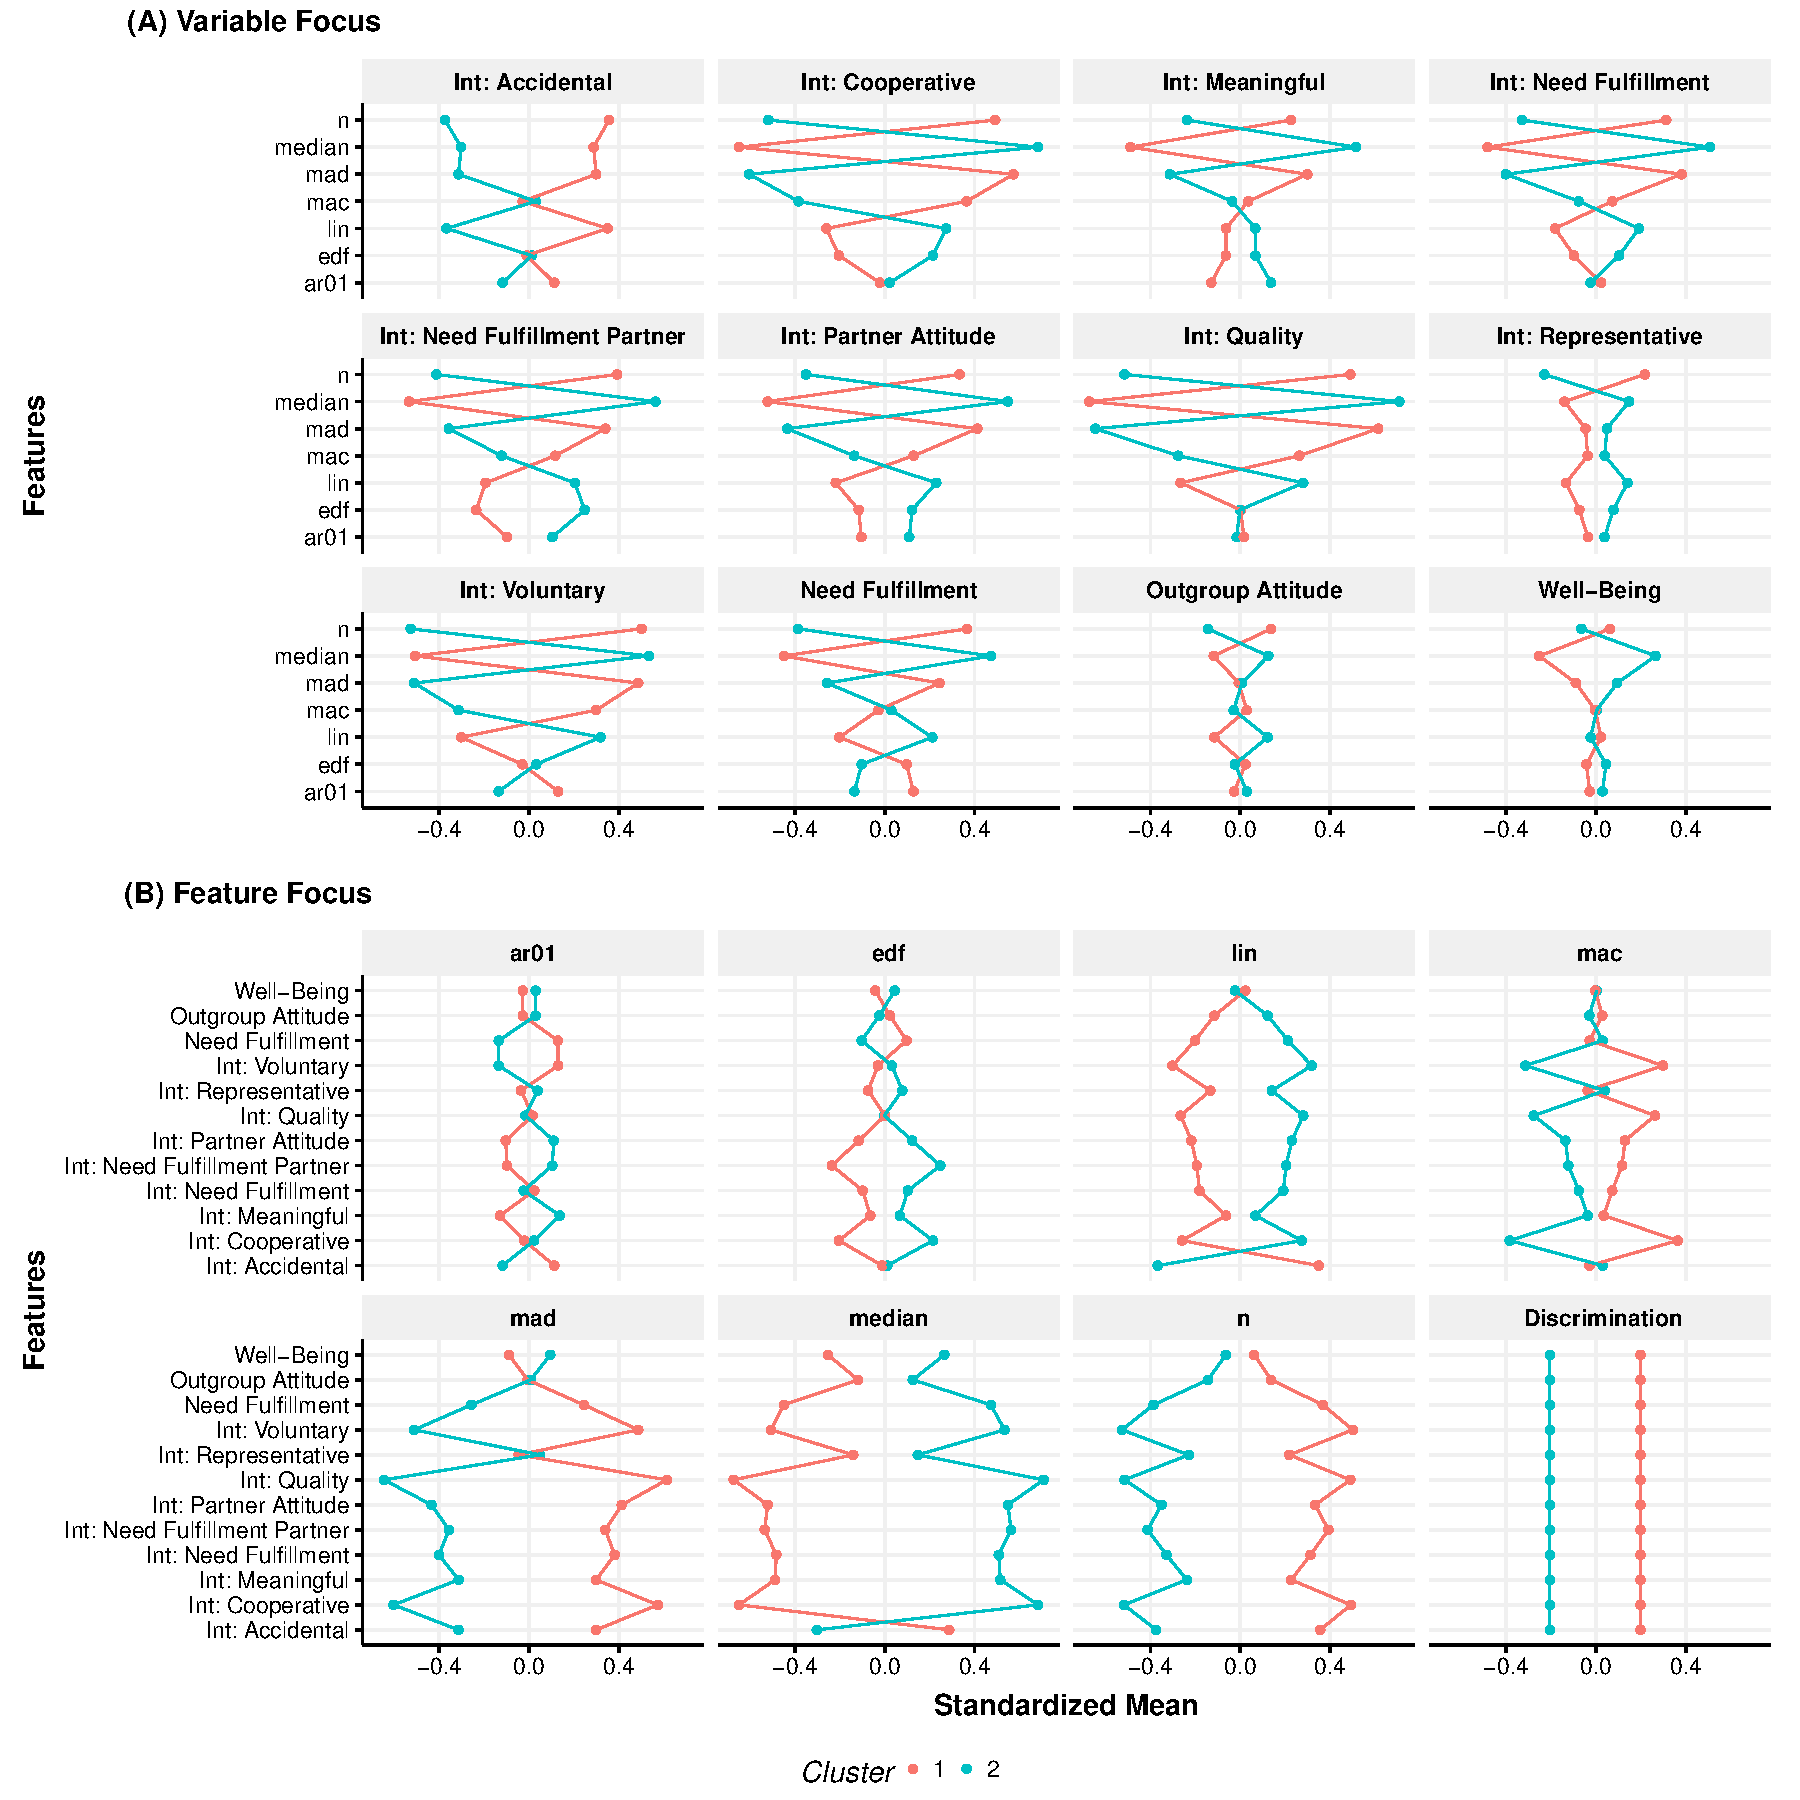
\includegraphics[width=\textwidth]{figures/clusterFeatVarComb.pdf}
  \caption*{Note: \\
  "Int." = outgroup interaction. Within the "(B) Feature Focus" subplot, the 'n' and 'Discrimination' comparison variables were not part of the original time series clustering.}
\end{figure}

In the second step, we look at the prototypical trajectories of the
clusters. For k-means clustering it is often recommended to use the
average over time of the responses within the cluster
\citep[see \fgrref{fig:clusterTs};][]{niennattrakul2007}\footnote{It is important to note, however, that direct comparability can be a concern, and often times some subset selection or nonlinear alignment is necessary \citep[e.g.,][]{gupta1996}. Additionally, finding cluster prototypes is often substantially easier with embedded clustering methods because in many cases a cluster-level model is estimated as part of the expectation–maximization procedure \citep[e.g.,][]{denteuling2021} or \textit{S-GIMME} \citep[e.g.][]{lane2019}. For medoid-based clustering algorithms, a common approach is simply using cluster medoid as the prototype \citep{kaufman1990}.}.
Immediately striking are the mean differences, where participants in
cluster 1 had more meaningful and fulfilling outgroup interactions and
also consistently reported more voluntary and cooperative interactions
but fewer accidental and involuntary interactions. The same cluster
(cluster 1) also reported an increase in need-fulfilling interactions
over the 30-day period and an increase in interactions that were
representative of the outgroup. Whereas the other cluster (cluster 2)
showed a decrease in voluntary, cooperative, and positive interactions
over the 30 days. This `deterioration' cluster (cluster 2) also saw a
decrease in general need fulfillment and experienced well-being over the
30 days (see \fgrref[B]{fig:clusterTs}). We also see that while
interaction representativeness, outgroup attitudes, and well-being are
relatively stable for both clusters, the deteriorating cluster (cluster
2) also showed substantially higher variability and instability on most
of the other variables (also see \fgrref[A]{fig:clusterTs}).

Finally, we can also assess the clusters across other individual
difference variables \citep[e.g.,][]{monden2022}. This out-of-feature
comparison allows us to check for data artifacts, as well as check
whether the developmental clusters are associated with important social
markers and individual differences. To illustrate artifact checks, we
added the number of ESM measurements into the comparison and find that
the participants in the deterioration cluster (cluster 2) on average
completed slightly more ESM surveys in general and reported on more
intergroup interactions in particular (see \(n\) in
\fgrref[B]{fig:clusterFeatVar}). In our data exclusion procedures, we
ensured that the general time frame and completion rates are similar for
all participants and indeed the numbers in ESM measurements generally
are largely similar (e.g., see \(n\) for well-being and outgroup
attitudes). However, the difference in the reported number of
interactions might indicate either a clustering artifact or a meaningful
difference. The higher average number of interactions in cluster 2
could, for example, indicate a clustering artifact if variances are more
inflated due to the larger samples \citep{kogan2006}. In our case this
seems less likely because one out of four variables did not differ in
terms of the MAD (see \fgrref{fig:cluster_comparison_mad}). At the same
time, however, the difference in the number of experienced interactions
might also indicate a meaningful difference, where the deteriorating
cluster (cluster 2) on average reported more outgroup interactions
(\textit{difference} = 1.03, \(t\)(150.83) = 7.50, \(p\) \textless{}
.001, \textit{95\%CI} {[}0.76, 1.30{]}), but these interactions were
less voluntary (\textit{difference} = -1.04, \(t\)(108.89) = -7.71,
\(p\) \textless{} .001, \textit{95\%CI} {[}-1.31, -0.77{]}), less
meaningful (\textit{difference} = -1.00, \(t\)(136.40) = -7.16, \(p\)
\textless{} .001, \textit{95\%CI} {[}-1.28, -0.73{]}), and less positive
(\textit{difference} = -1.38, \(t\)(152.31) = -11.94, \(p\) \textless{}
.001, \textit{95\%CI} {[}-1.61, -1.15{]}). Such a finding is in line
with past research highlighting the role of negative intergroup
interactions in explaining intergroup relations
\citep[e.g.,][]{Barlow2012, Prati2021, Graf2014}.

\begin{figure}[!ht] %hbtp
  \caption{Cluster comparison of Median Absolute Deviation for all variables}
  \label{fig:cluster_comparison_mad}
  \centering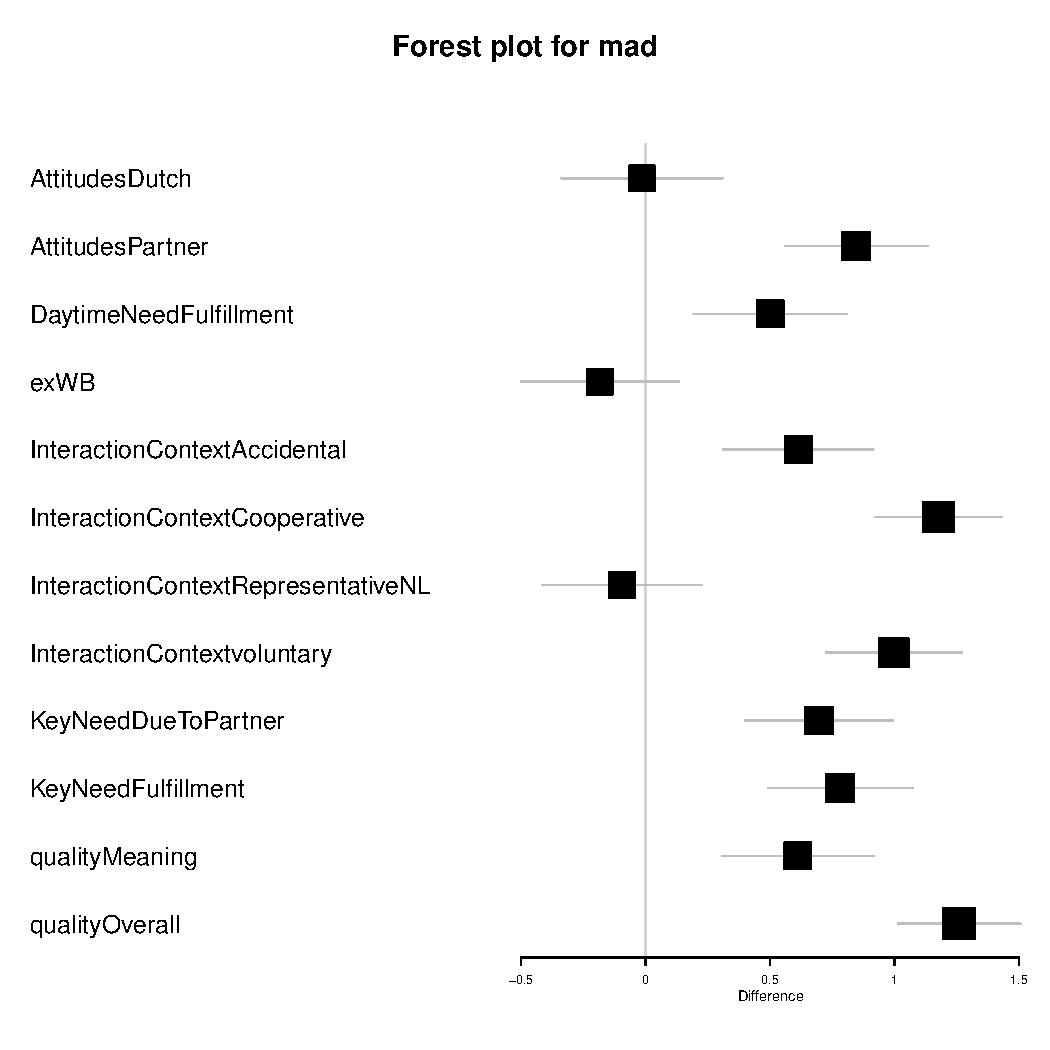
\includegraphics[width=\textwidth]{figures/feature_comparison_mad.pdf}
\end{figure}

To further illustrate the utility of assessing out-of-feature individual
differences, we also compare the two samples in terms of the
participants' self-reported discrimination experiences in the
Netherlands (measured during the post-measurement). When looking at the
group comparison, we find that participants in the deteriorating cluster
(cluster 2) reported substantially higher levels of everyday
discrimination (\fgrref[B]{fig:clusterFeatVar}). Thus, both intensive
longitudinal (e.g., the sum of specific ESM measurements) and
cross-sectional variables (e.g., general discrimination differences)
that were not included in the original clustering step can be used to
explore and understand the cluster differences in more detail.

This cluster separation, then, has a number of empirical and practical
applications. Firstly, the clusters are descriptive. With tens of
variables, hundreds of participants, and thousands of measurements,
singular descriptive statistics are often not able to capture the
complex patterns that describe the data set. The feature-based
clustering offers some direct insight into the complexity within the
data set. In our empirical example, we, for example, see that
participants are meaningfully distinguished by a combination of high
(vs.~low) central tendency, variability, and linear trend. Secondly, the
clusters identify important groups. The adaptive and deteriorating
groups offer starting points for empirical exploration as well as
practical interventions. Researchers can start probing what exactly
distinguishes the two groups further and generate new bottom-up
hypotheses. Practitioners in the resettlement field can use the group
separation to identify individuals in need of assistance and can explore
contextual factors that might contribute to the difficulties some might
face. In our illustration we, for example, found that participants in
the deteriorating cluster (cluster 2) reported less need fulfilling
interactions over time. Thirdly, the feature-based approach is flexible
and meaningful. We were able to use a wide range of time series features
that have been central in the ESM literature and were able to use them
directly to identify meaningful groups. For our empirical illustration
we, among others for example, chose to focus on whether participants
differed in their average well-being (i.e., \textit{median}), how much
their well-being would vary over time (i.e, \textit{MAD}), and whether
their well-being would on average increase or decrease over time (i.e.,
\textit{linear trend}). Alternatively, for others cyclical patterns
might be more important --- for example, whether well-being was higher
on weekends. Importantly, in any case, we did not need to translate
these dynamic features into probabilistic inference models (e.g., VAR
models) to cluster the participants.

\begin{figure}[!ht] %hbtp
  \caption{Cluster Group Comparisons over time}
  \label{fig:clusterTs}
  \centering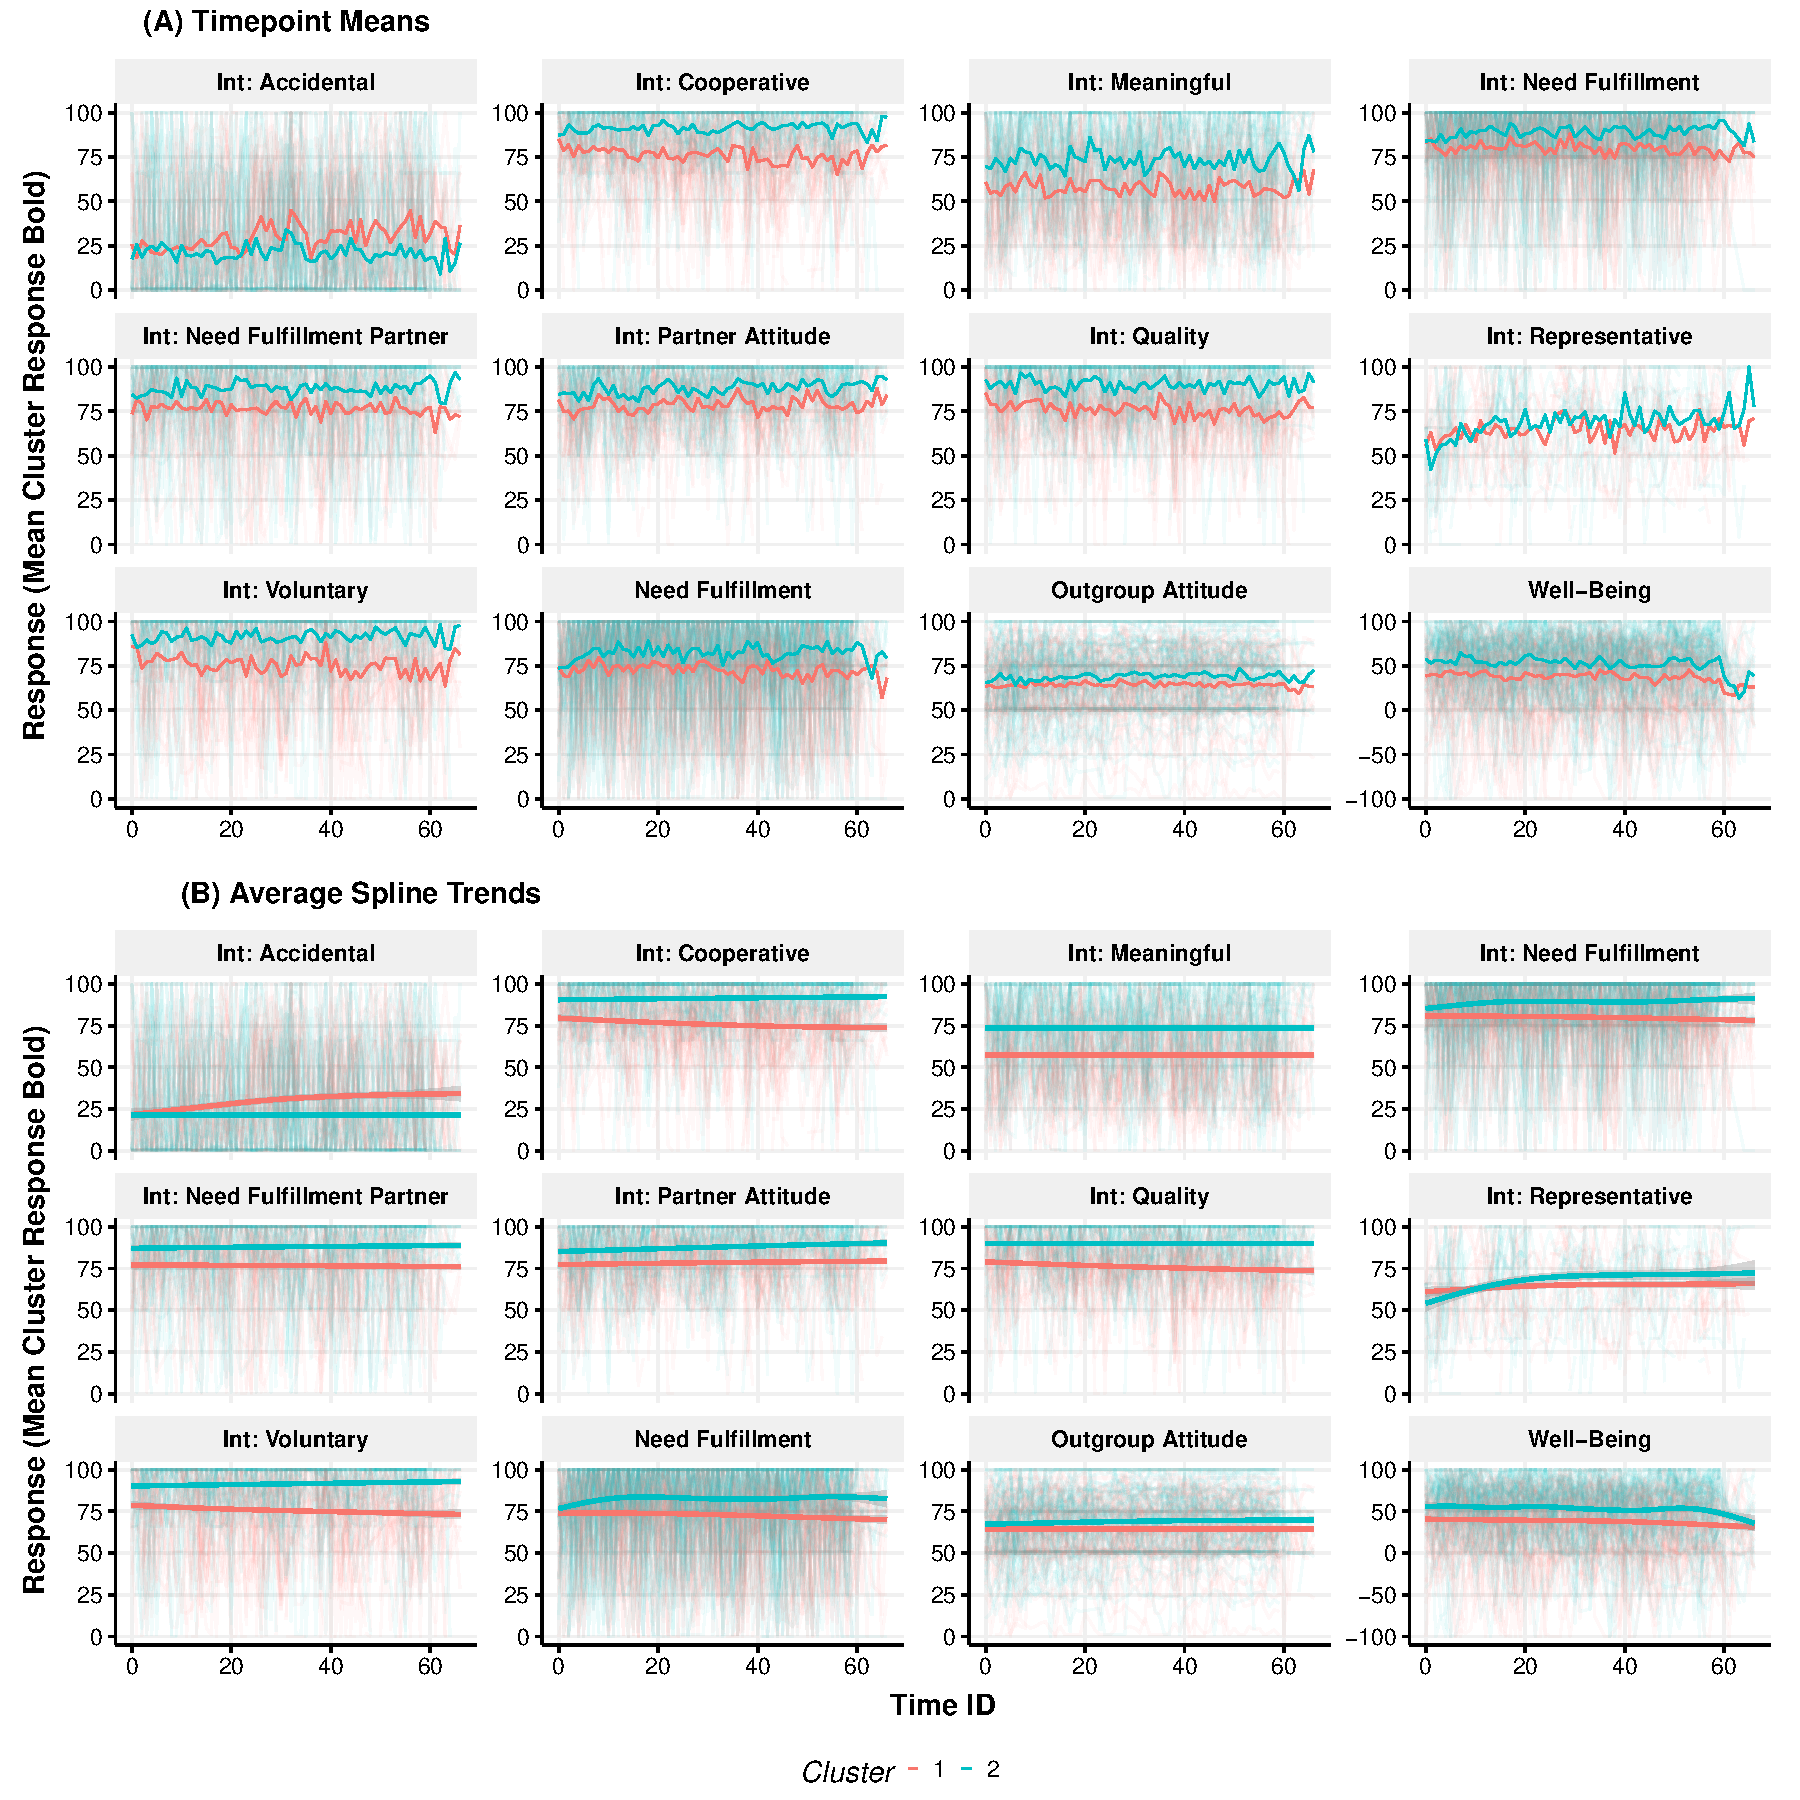
\includegraphics[width=\textwidth]{figures/clusterTsComb.pdf}
  \caption*{Note: \\
  Subplot (A) displays the variable cluster means at every measurement occasion. Subplot (B) shows the GAM spline for each cluster across the measurement occasions. The thinner lines present all individual time series.}
\end{figure}
